\documentclass{article}
\usepackage[utf8]{inputenc}
\usepackage[a4paper, margin=1in]{geometry}
\usepackage{fancyhdr}
\usepackage{titlesec}
\usepackage[backend=bibtex,style=verbose-trad2]{biblatex}
\usepackage{hyperref}
\usepackage{graphicx}
\usepackage{algorithm}
\usepackage{algpseudocode}
\usepackage{float}
\usepackage{multicol}
\usepackage{url}

\addbibresource{references.bib}

\title{Kernel Image Processing}
\author{Luka Uršič \\ 89221145 \\ UP Famnit \\ E-mail: 89221145@student.upr.si}
\date{\today}

\pagestyle{fancy}
\fancyhf{}
\rhead{\today}
\lhead{Kernel Image Processing}
\rfoot{Page \thepage}
\titleformat{\section}
{\normalfont\Large\bfseries}{\thesection}{1em}{}

\begin{document}

\maketitle
\thispagestyle{empty}

\begin{abstract}
    In this paper, I present how to use kernel image processing to modify an image. I explain how kernel image processing works, how I implemented it, and the time results I obtained from running it sequentially, in parallel, and with distributed computing. I compare the results and conclude which method is the best for this specific task.
\end{abstract}

\begin{multicols}{2}

    \section{Introduction}
    An image kernel is a small matrix used to apply effects like the ones you might find in popular photo manipulation software, such as blurring, sharpening, outlining, or embossing. They're also used in machine learning for 'feature extraction', a technique for determining the most important portions of an image. In this context, the process is referred to more generally as "convolution".

    \cite{setosa}

    \section{Algorithm}

    Here is the mathematical definition of the convolution of original image $f$, kernel $\omega$, and resulting image $g$:

    \begin{equation}
        g(x, y) = \omega * f(x, y) = \sum_{i=-a}^{a} \sum_{j=-b}^{b} \omega(i, j) f(x-i, y-j)
    \end{equation}

    \cite{wikipedia}

    \vfill

    To perform a convolution, the program uses a kernel, which is essentially a small matrix that is applied to each pixel in the image. This kernel works by interacting with the pixel and its surrounding neighbors. The new value of the pixel is calculated through a process where the kernel is multiplied by the surrounding pixels, and the resulting values are summed up.

    \begin{figure}[H]
        \centering
        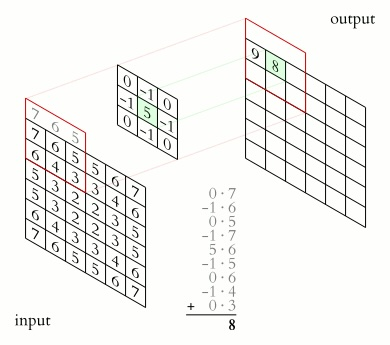
\includegraphics[width=\linewidth]{img/kernel.jpg}
        \caption{Convolution of an image with a kernel}
        \label{fig:Kernel}
    \end{figure}

    This technique is used in various image processing tasks, such as blurring, sharpening, edge detection, and more. By systematically applying the kernel across the entire image, the program can achieve the desired transformation or effect, that can be used in image manipulation programs or machine learning algorithms.

    This process is usualy done sequentially, pixel by pixel, row by row. Now imagine that we have a large image with millions of pixels. This process can take a long time. To speed up the process, we can use parallel computing. We can split the image into smaller parts and process them in parallel. This way, we can process the image much faster.

    \section{Implementation}
    I implemented Kernel Image Processing in Java and used the Swing and AWT libraries to display the images.

    I created a class called ImageProcessor that contains the methods applyKernelToPixel, applyKernel, applyKernelSequential, and applyKernelParallel. The applyKernelToPixel method applies the kernel to a single pixel, the applyKernel method applies the kernel to the entire image, the applyKernelSequential method applies the kernel to the image sequentially, and the applyKernelParallel method applies the kernel to the image in parallel.

    You can see the pseudocode for the class ImageProcessor in the following algorithm.

    \begin{algorithm}[H]
        \caption{Pseudocode for ImageProcessor.java}
        \begin{algorithmic}[1]
            \State \textbf{Class} ImageProcessor
            \State \textbf{Function} applyKernelToPixel(image, kernel, result, x, y)
            \For{each value in the kernel}
            \State Multiply the corresponding pixel color by the kernel value
            \State Add the result to r, g, b
            \EndFor
            \State Clamp r, g, b between 0 and 255
            \State Set the pixel in the result image to the new color
            \State \textbf{End Function}
            \State
            \State \textbf{Function} applyKernel(image, kernel)
            \For{each pixel in the image}
            \State Apply the kernel to the pixel
            \EndFor
            \State \textbf{End Function}
            \State
            \State \textbf{Function} applyKernelSequential(image, kernel)
            \State Apply the kernel to the image
            \State Return the result image
            \State \textbf{End Function}
            \State
            \State \textbf{Function} applyKernelParallel(image, kernel)
            \State Use a ForkJoinPool to apply the kernel to each pixel in parallel
            \State Return the result image
            \State \textbf{End Function}
            \State \textbf{End Class}
        \end{algorithmic}
    \end{algorithm}

    \subsection{Sequential}

    The applyKernelSequential method processes each pixel in the image one by one, row by row. This method is simple and easy to implement, but it can be slow for large images.

    \subsection{Parallel}

    The applyKernelParallel method applies the kernel to the image in parallel using a ForkJoinPool. This method splits the image into smaller parts and processes them in parallel. This approach can be much faster than the sequential method, especially for large images.

    \begin{figure}[H]
        \centering
        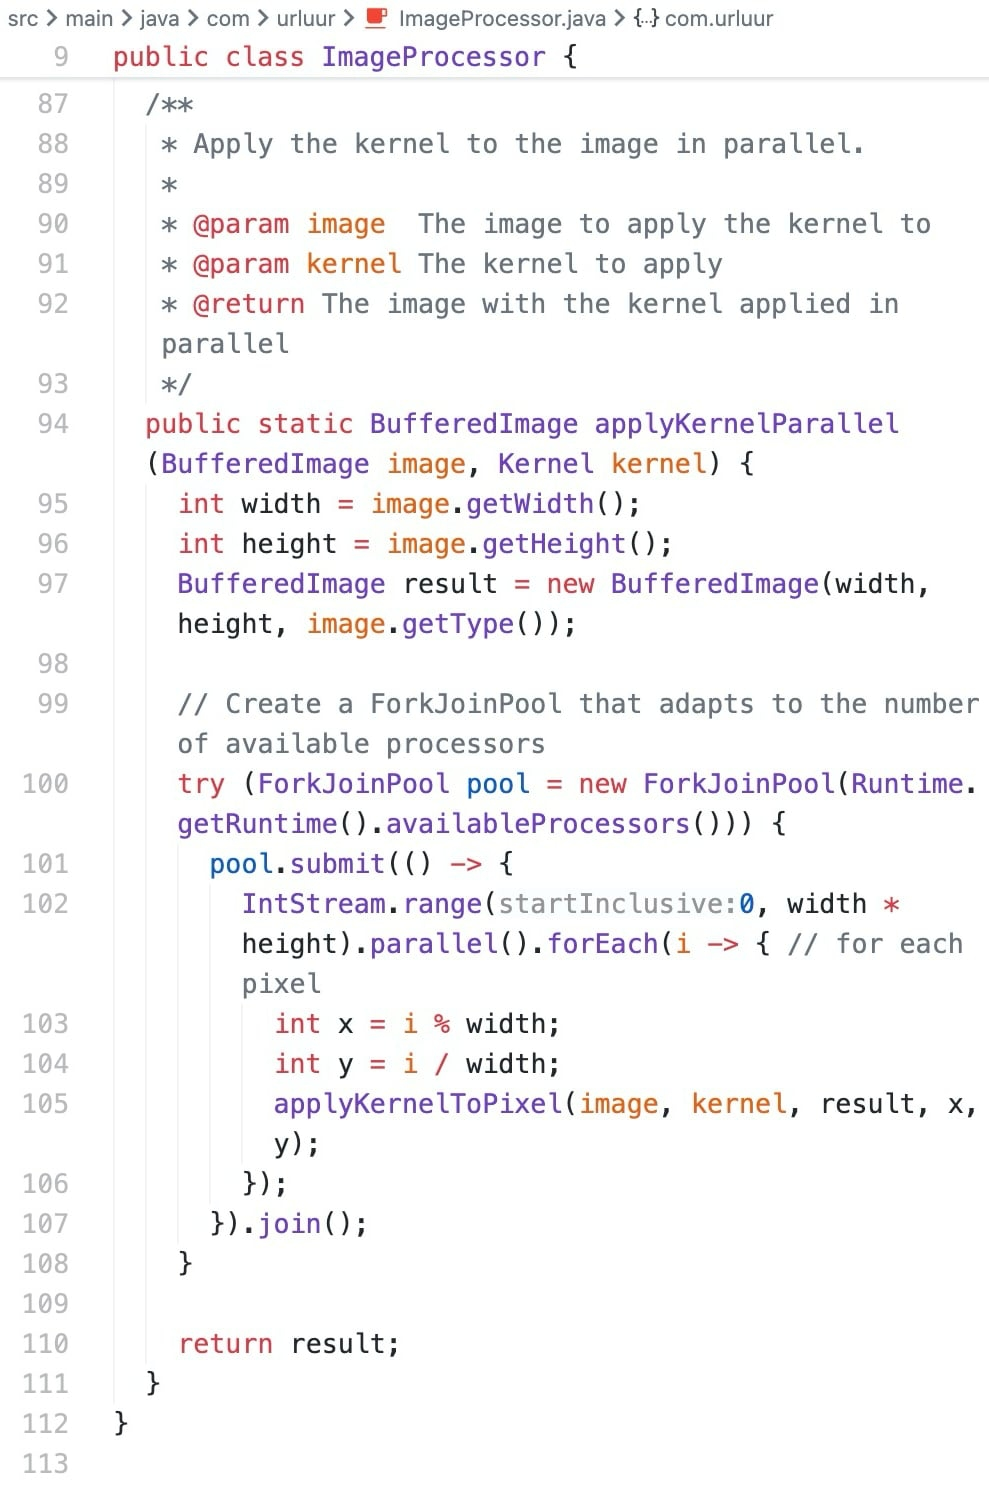
\includegraphics[width=\linewidth]{img/parallel.jpg}
        \caption{Code for parallel processing}
        \label{fig:Parallel Code}
    \end{figure}


    % \subsection{Distributed}





    \section{Results}

    I tested the program on my computer in sequential mode and in parallel mode with three pictures of different sizes. Results in sequential mode were following the number of pixels in the image. The results in parallel mode were faster than in sequential mode. The difference was significant. It noted speedups of up to 4x. What surprised me is that the speedup was present with small and large images.

    \begin{figure}[H]
        \centering
        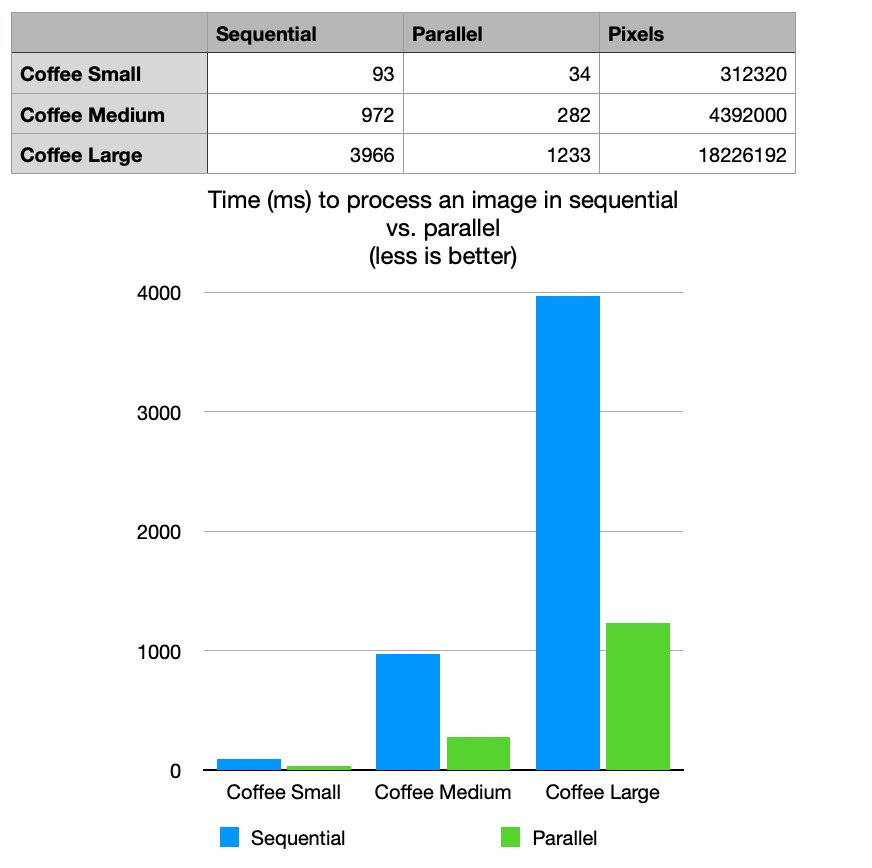
\includegraphics[width=\linewidth]{img/coffee_speedup.jpg}
        \caption{Speedup comparison between sequential and parallel processing}
        \label{fig:speedup}
    \end{figure}

    What was even more surprising to me is the fact that the distributed computing was slower than the parallel computing. I expected the distributed computing to be faster, but it was slower. The reason for this is that the overhead of sending the image to the other machines was too high.

    \section{Conclusion}

    The results of my experiments show that parallel computing using a ForkJoinPool provides significant speedup compared to sequential processing. The speedup was observed for both small and large images, indicating that parallel processing is beneficial regardless of image size.

    However, the distributed computing approach did not yield better performance compared to parallel computing. The overhead of sending the image to other machines outweighed the potential benefits of distributed processing.

\end{multicols}

\printbibliography[heading=bibintoc, title={References}]

\end{document}